\documentclass{article}

\usepackage{listings}
\usepackage{enumitem}
\usepackage{amsmath}
\usepackage{svg}
\usepackage{hyperref}
\hypersetup{
    colorlinks=true,
    linkcolor=blue,
    filecolor=magenta,      
    urlcolor=cyan,
    pdftitle={Overleaf Example},
    pdfpagemode=FullScreen,
    }

\title{CA Lab: Lab 6}
\author{student: Dimitri Tabatadze}

\newcommand{\points}[1]{{\footnotesize{\color{red}\textit{#1 points}}}}

\definecolor{codegreen}{rgb}{0,0.6,0}
\definecolor{codegray}{rgb}{0.5,0.5,0.5}
\definecolor{codepurple}{rgb}{0.58,0,0.82}
\definecolor{backcolour}{rgb}{0.98,0.96,0.94}

\lstdefinestyle{mystyle}{
    backgroundcolor=\color{backcolour},   
    commentstyle=\color{codegreen},
    keywordstyle=\color{magenta},
    numberstyle=\tiny\color{codegray},
    stringstyle=\color{codepurple},
    basicstyle=\ttfamily\footnotesize,
    breakatwhitespace=false,         
    breaklines=true,                 
    captionpos=b,                    
    keepspaces=true,                 
    numbers=left,                    
    numbersep=5pt,                  
    showspaces=false,                
    showstringspaces=false,
    showtabs=false,                  
    tabsize=2
}

\lstset{style=mystyle}

\begin{document}
    \maketitle

    \section*{Task Description} 
    
    Design of Clock divider, where the input clock is divided by an odd integer.

    \begin{enumerate}
        \item Draw the circuits. \points{10}
        \item Write the equation. \points{10}
        \item Write and test the code. \points{70} (main file \points{40}, run to the board-\points{30})
    \end{enumerate}

    Please, solve the problems (write the comments) \points{5}, take the clear screenshots and combine all your solutions in one pdf file, then upload in teams. \points{5}

    \section*{Solution}

    \begin{enumerate}
        \item {
            The circuit diagram:

            \begin{figure}[h]
                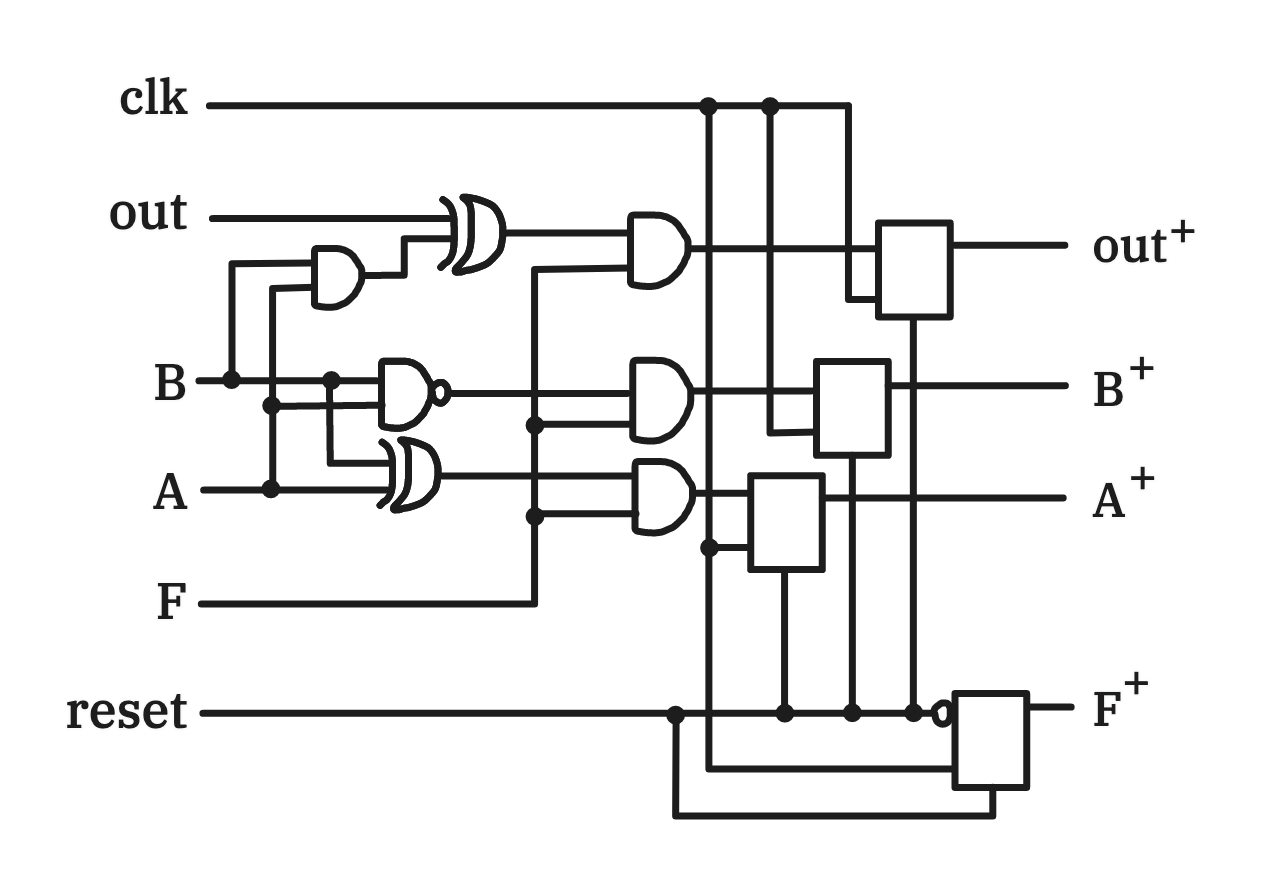
\includegraphics[width=7cm]{diagram.png}
            \end{figure}
        }
        \item {
            The equations
        
            \begin{displaymath}
                \begin{aligned}
                    A^+ &= F \land (A \oplus B) \\
                    B^+ &= F \land \overline{(A \land B)} \\
                    \text{out}^+ &= F \land (\text{out} \oplus (A \land B)) \\
                    F^+ &= \overline{reset}
                \end{aligned}
            \end{displaymath}
        }
        \item {
            The Verilog code:

            \begin{lstlisting}[language=verilog]
module divider (
    input clock,
    input reset,
    output reg out = 0
);

reg A = 0;
reg B = 0;
reg F = 0;

always @(clock, posedge reset) begin
    if (~reset) begin
        A <= F & (A ^ B);
        B <= F & ~(A & B);
        out <= F & (out ^ (A & B));
        F <= ~reset;
    end else begin
        A <= 0;
        B <= 0;
        F <= 0;
        out <= 0;
    end
end

endmodule\end{lstlisting}
        }
    \end{enumerate}

    \section*{Conclusion}
    
    This task took me more time than I would have prefered it to. I can assure you, this code works, here's the timing diagram along with a testbench:
    
    \begin{lstlisting}[language=verilog]
module divider_tb();

reg clock;
reg reset;
wire out;

divider UUT(.clock(clock), .reset(reset), .out(out));

always #2 clock = ~clock;

initial begin
    clock = 0;
    reset = 0;
    #20;
    reset = 1;
    #19;
    reset = 0;
    #20;
    $finish;
end

endmodule\end{lstlisting}

    \begin{figure}[h]
        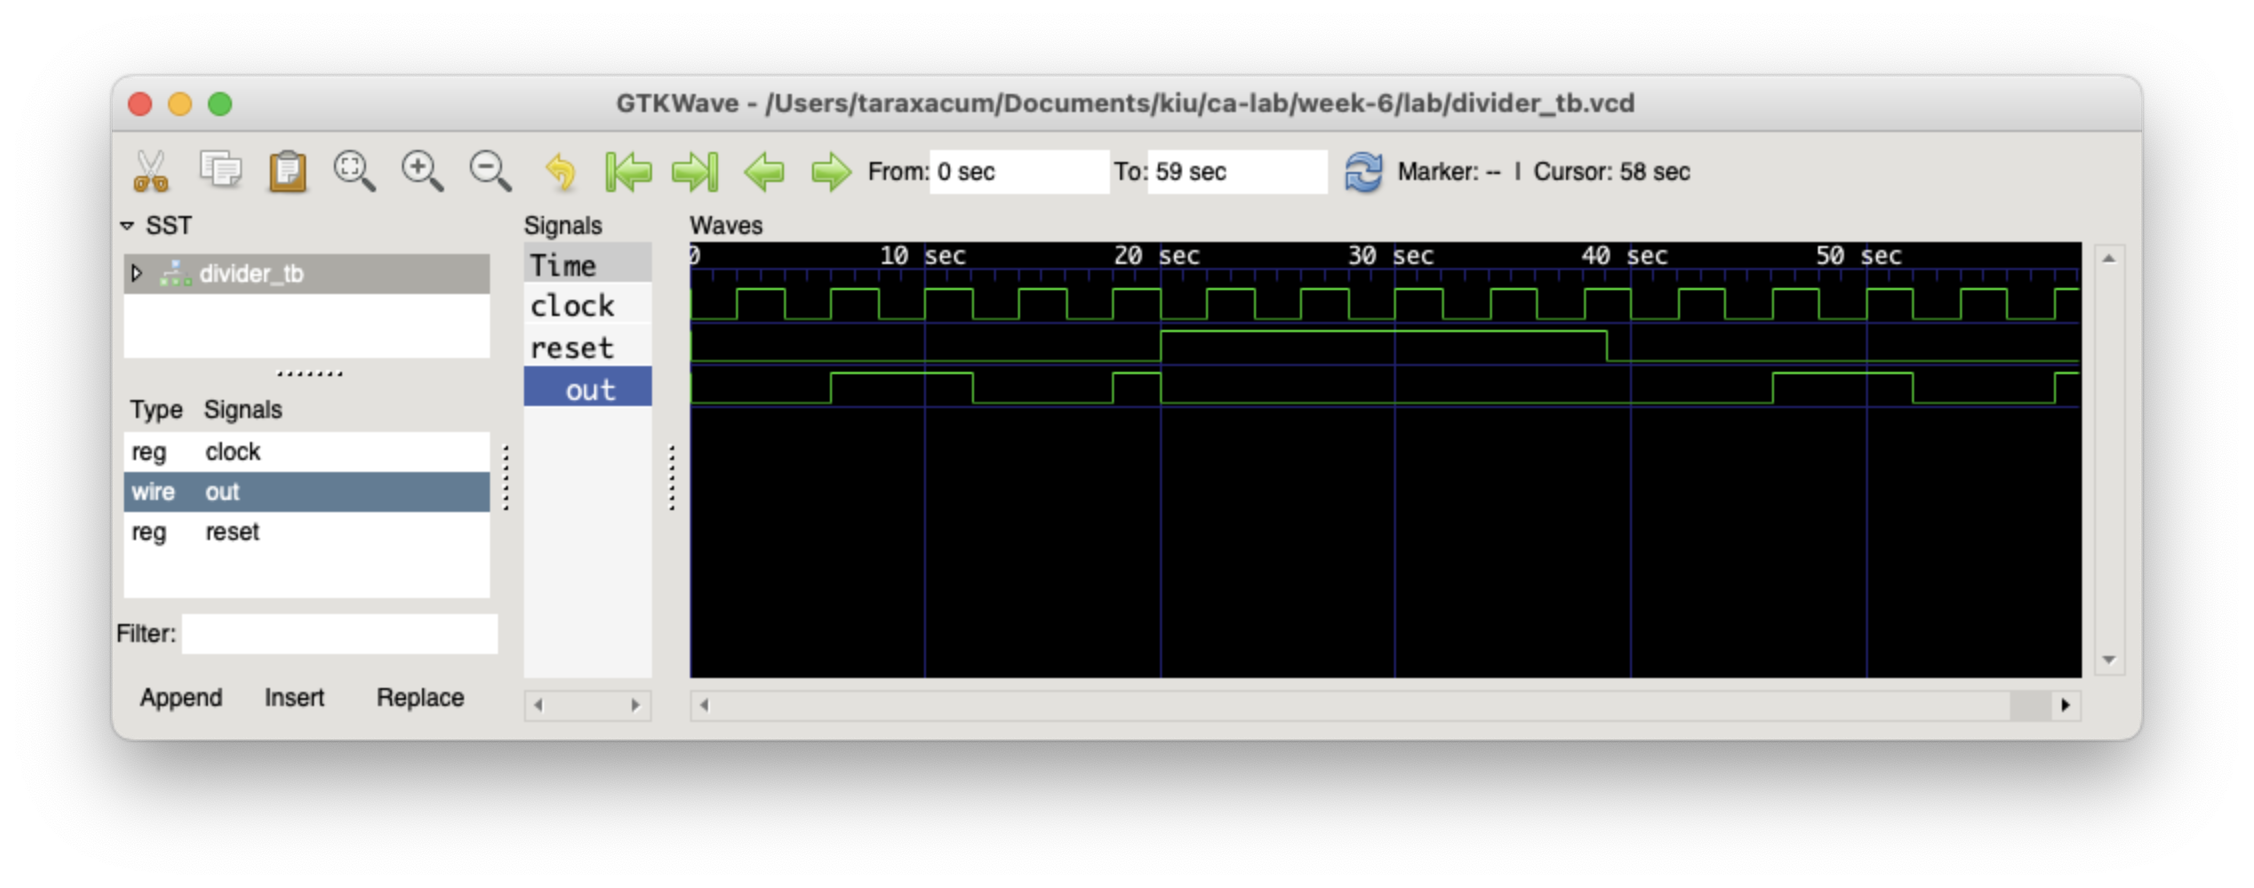
\includegraphics[width=12cm]{timing-diagram.png}
    \end{figure}
    
    \section*{Reference}
    
    \begin{itemize}
        \item My whiteboard
    \end{itemize}

\end{document}